\section{``SIMD for nothin', FLOPS for free'' (old song)}

\begin{frame}{SIMD}
	\begin{itemize}
		\item SIMD = ``simple instruction, multiple data'' (in Flynn's taxonomy). Correspond to data level parallelism.
		\item Refers to (at least) two mechanisms: pipelining\footnote{See ``Fonctions et concepts des ordinateurs'' (INFOB2126/IHDCB142)} and \textbf{packed instruction} / vector processing.
		\item Response to early graphic cards: MMX (64 bits registers, for integers) / 3DNow! (+\cdx{float}) \textrightarrow{} SSE (128 bit registers, +\cdx{double}) \textrightarrow{} AVX (256 and 512 bit registers)
		\item Example: SSE\begin{center}
			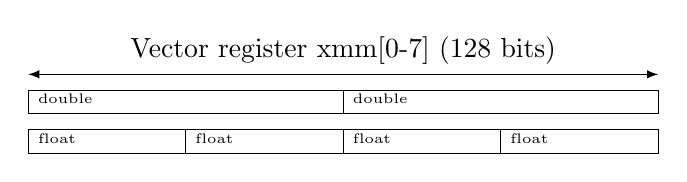
\begin{tikzpicture}
				\draw[latex-latex] (0,0) -- +(8,0) node[midway,above]{Vector register \cdx{xmm[0-7]} (128 bits)};
				\draw (0,-.5) node[anchor=south west]{\tiny \cdx{double}} rectangle +(4,.3);
				\draw (4,-.5) node[anchor=south west]{\tiny \cdx{double}} rectangle +(4,.3);
				\draw (0,-1) node[anchor=south west]{\tiny \cdx{float}} rectangle +(2,.3);
				\draw (2,-1) node[anchor=south west]{\tiny \cdx{float}} rectangle +(2,.3);
				\draw (4,-1) node[anchor=south west]{\tiny \cdx{float}} rectangle +(2,.3);
				\draw (6,-1) node[anchor=south west]{\tiny \cdx{float}} rectangle +(2,.3);
			\end{tikzpicture}
		\end{center}
	\end{itemize}
\end{frame}

\begin{frame}[fragile]{Vector processing}
	Examples with SSE (as modified by AVX):
	\begin{ccode}
float x[N], y[N], z[N];
for(i=0; i < N; i++)
	z[i] = x[i] + y[i];
	\end{ccode}
	The last line is translated into \texttt{vaddps} \textcolor{blue}{\texttt{xmm1}},\textcolor{red}{\texttt{xmm2}},\textcolor{green}{\texttt{xmm3}} (among other things).
	\begin{center}
		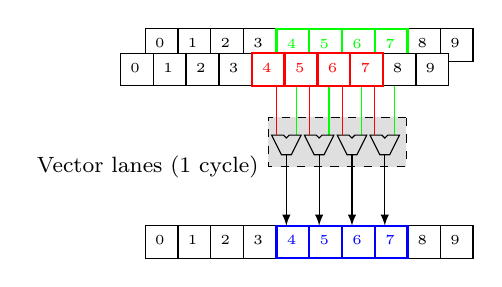
\begin{tikzpicture} [scale=1.25,rotate=-90]
			\draw[dashed,fill=gray!25] (.9,2.65)  rectangle +(.5,-1.4)node[left]{\footnotesize Vector lanes (1 cycle)};
			\foreach\i in {0,1,2,3,8,9} {
				\draw (0,\i / 3) node[anchor=north west]{\tiny \i} rectangle +(.33,.33);	
				\draw (2,\i / 3) node[anchor=north west]{\tiny \i} rectangle +(.33,.33);
			}
			\foreach\i in {4,5,6,7} {
				\draw[green,thick] (0,\i / 3) node[anchor=north west]{\tiny \i} rectangle +(.33,.33);	
				\draw[blue,thick] (2,\i / 3)  node[anchor=north west]{\tiny \i} rectangle +(.33,.33);
				\draw[green] (.33,\i / 3 + .2) -- ++(.75,0);
				\draw (1.08, \i / 3 + .25) -- ++(.2,-.1) -- ++(0,-.1) -- ++(-.2,-.1)  -- ++(0,.12)-- ++(.03,.03) -- ++(-.03,.03) -- cycle;
				\draw[-latex] (1.28,\i / 3 + .1) -- (2,\i / 3 + .1);
			}
			\foreach\i in {0,1,2,3,8,9} {
				\draw[fill=white] (.25,\i / 3 - .25) node[anchor=north west]{\tiny \i} rectangle +(.33,.33);
			}
			\foreach\i in {4,5,6,7} {	
				\draw[red,fill=white,thick] (.25,\i / 3 - .25) node[anchor=north west]{\tiny \i} rectangle +(.33,.33);
				\draw[red] (.58,\i / 3) -- ++(.5,0); 
			}
		\end{tikzpicture}
	\end{center}
	The program runtime for this part is (theoretically!) divided by the number of vector lanes.
\end{frame}

\begin{frame}[fragile]{Howto!}
	\begin{itemize}
		\item Write assembler (\textbf{don't!})
		\item Use compiler intrinsic (if you \textbf{really} have to):\begin{ccode}
#include <xmmintrin.h>
__m128 r1 = _mm_load_ps(&x[4*i]);
__m128 r2 = _mm_load_ps(&y[4*i]);
__m128 r0 = _mm_add_ps(r1, r2);
_mm_store_ps(&z[4*i],r0);
		\end{ccode}
		\item Use SIMD classes (in C++)
		\item Add \cdx{\#pragma omp simd} above the loop (other exists, but it depends on the compiler) and compile with \cdx{-fopenmp-simd} (gcc).
		\item Let the compiler do its job ... And maybe check its result. With gcc, \cdx{-ftree-vectorize} (or \cdx{-O2}) and \cdx{-fopt-info-loop-(optimized|missed)}. The compiler may refuse to optimize a loop, though.
	\end{itemize}
\end{frame}

\begin{frame}[fragile]{Aliasing?}
	
	\begin{itemize}
		\item If one compiles the serial code of the \cdx{axpy} example, the output is something like\begin{textcode}
1_serial.c:11:9: optimized: loop vectorized using 16 byte
vectors
1_serial.c:11:9: optimized:  loop versioned for 
vectorization because of possible aliasing
(...)
		\end{textcode}
		So the loop (here the one of \cdx{saxpy}) get vectorized (with 16-byte vector, so a 128 bit register), but also versioned.
		\item Here, the compiler is not able to determine whether \cdx{x} and \cdx{y} point to the same memory address, so it keeps both versions (and will choose at runtime).
		\item Use \cdx{restrict} to help:\begin{ccode}
void saxpy(int n, float alpha, 
	float* restrict x, float* restrict y) 
		\end{ccode}
	\end{itemize}
\end{frame}

\begin{frame}{Results}
	\begin{table}
		\begin{tabular}{p{4.5cm}lll}
			\toprule
			&Instruction& \cdx{saxpy} & \cdx{daxpy} \\
			\midrule
			\cdx{\small -O1} & \cdx{mulsd} & 30.7 & 31.7 \\
			\cdx{\small -O1 -ftree-vectorize} & \cdx{mulpd} & 16.0 & 27.3 \\
			\cdx{\small -O1 -lm -ftree-vectorize -mavx2} & \cdx{vmulpd} + 2 l.u. & 16.2 & 27.3 \\
			\cdx{\small -O1 -ftree-vectorize \mbox{-m}arch=native -mtune=native}  & \cdx{vmulpd} + 4 l.u. & 14.5 & 25.8 \\
			\bottomrule
		\end{tabular}
	\caption{Instruction for multiplication of double and average running times (in ms) with \cdx{-N 1000}, on $2^{24}$ numbers.}
	\end{table}
\begin{itemize}
	\item Use \cdx{-march=native -mtune=native} for best performances.
	\item \cdx{dot} does not vectorize ... \textbf{Why?}
\end{itemize}
\end{frame}